\chapter{位运算}

计算机程序中的所有数据在内部都以比特（bit）的形式存储，
即以数字0和1的形式存储。
本章讨论整数的位表示，
并给出如何使用位运算的示例。
事实证明，位运算在算法编程中有着许多用途。

\section{位表示}

\index{位表示}

在编程中，一个 $n$ 位整数在内部以
由 $n$ 个比特组成的二进制数的形式存储。
例如，C++类型 \texttt{int} 是一个32位类型，
这意味着每个 \texttt{int} 数由32个比特组成。

以下是 \texttt{int} 数43的位表示：
\[00000000000000000000000000101011\]
表示中的比特从右到左进行编号。
要将一个位表示 $b_k \cdots b_2 b_1 b_0$ 转换为数字，
我们可以使用以下公式
\[b_k 2^k + \ldots + b_2 2^2 + b_1 2^1 + b_0 2^0.\]
例如，
\[1 \cdot 2^5 + 1 \cdot 2^3 + 1 \cdot 2^1 + 1 \cdot 2^0 = 43.\]

一个数的位表示要么是\key{有符号}的（signed），要么是\key{无符号}的（unsigned）。
通常使用有符号表示，
这意味着负数和正数都可以被表示。
一个 $n$ 位的有符号变量可以包含
$-2^{n-1}$ 和 $2^{n-1}-1$ 之间的任何整数。
例如，C++中的 \texttt{int} 类型是有符号类型，
因此一个 \texttt{int} 变量可以包含
$-2^{31}$ 和 $2^{31}-1$ 之间的任何整数。

在有符号表示中，第一个比特是数字的符号位
（0表示非负数，1表示负数），
其余的 $n-1$ 个比特包含数字的大小。
使用的是\key{二进制补码}（Two's complement），
这意味着一个数的相反数是通过
先将该数的所有位取反，
然后再将数加一来计算的。

例如，\texttt{int} 数 $-43$ 的位表示是
\[11111111111111111111111111010101.\]

在无符号表示中，只能使用非负数，
但值的上界更大。
一个 $n$ 位的无符号变量可以包含
$0$ 和 $2^n-1$ 之间的任何整数。
例如，在C++中，\texttt{unsigned int} 变量
可以包含 $0$ 和 $2^{32}-1$ 之间的任何整数。

这两种表示之间存在联系：
有符号数 $-x$ 等于无符号数 $2^n-x$。
例如，以下代码显示
有符号数 $x=-43$ 等于无符号数 $y=2^{32}-43$：
\begin{lstlisting}
int x = -43;
unsigned int y = x;
cout << x << "\n"; // -43
cout << y << "\n"; // 4294967253
\end{lstlisting}

如果一个数超出了位表示的上界，
该数就会溢出。
在有符号表示中，
$2^{n-1}-1$ 之后的下一个数是 $-2^{n-1}$，
而在无符号表示中，
$2^n-1$ 之后的下一个数是 $0$。
例如，考虑以下代码：
\begin{lstlisting}
int x = 2147483647
cout << x << "\n"; // 2147483647
x++;
cout << x << "\n"; // -2147483648
\end{lstlisting}

初始时，$x$ 的值是 $2^{31}-1$。
这是可以存储在 \texttt{int} 变量中的最大值，
因此 $2^{31}-1$ 之后的下一个数是 $-2^{31}$。


\section{位运算}

\newcommand\XOR{\mathbin{\char`\^}}

\subsubsection{与运算}

\index{与运算}

\key{与}（and）运算 $x$ \& $y$ 生成一个数，
该数在 $x$ 和 $y$ 都有1的位置上为1。
例如，$22$ \& $26$ = 18，因为

\begin{center}
\begin{tabular}{rrr}
& 10110 & (22)\\
\& & 11010 & (26) \\
\hline
 = & 10010 & (18) \\
\end{tabular}
\end{center}

利用与运算，我们可以检查一个数 $x$ 是否为偶数，
因为当 $x$ 为偶数时 $x$ \& $1$ = 0，
当 $x$ 为奇数时 $x$ \& $1$ = 1。
更一般地，$x$ 能被 $2^k$ 整除
当且仅当 $x$ \& $(2^k-1)$ = 0。

\subsubsection{或运算}

\index{或运算}

\key{或}（or）运算 $x$ | $y$ 生成一个数，
该数在 $x$ 和 $y$ 中至少一个为1的位置上为1。
例如，$22$ | $26$ = 30，因为

\begin{center}
\begin{tabular}{rrr}
& 10110 & (22)\\
| & 11010 & (26) \\
\hline
 = & 11110 & (30) \\
\end{tabular}
\end{center}

\subsubsection{异或运算}

\index{异或运算}

\key{异或}（xor）运算 $x$ $\XOR$ $y$ 生成一个数，
该数在 $x$ 和 $y$ 中恰好一个为1的位置上为1。
例如，$22$ $\XOR$ $26$ = 12，因为

\begin{center}
\begin{tabular}{rrr}
& 10110 & (22)\\
$\XOR$ & 11010 & (26) \\
\hline
 = & 01100 & (12) \\
\end{tabular}
\end{center}

\subsubsection{非运算}

\index{非运算}

\key{非}（not）运算 \textasciitilde$x$
生成一个将 $x$ 的所有位取反后的数。
公式 \textasciitilde$x = -x-1$ 成立，
例如，\textasciitilde$29 = -30$。

非运算在位级别的结果取决于位表示的长度，
因为该运算会将所有位取反。
例如，如果数字是32位的 \texttt{int} 数，
结果如下：

\begin{center}
\begin{tabular}{rrrr}
$x$ & = & 29 &   00000000000000000000000000011101 \\
\textasciitilde$x$ & = & $-30$ & 11111111111111111111111111100010 \\
\end{tabular}
\end{center}

\subsubsection{位移}

\index{位移}

左移 $x < < k$ 在数的末尾添加 $k$ 个零，
右移 $x > > k$ 移除数的最后 $k$ 个位。
例如，$14 < < 2 = 56$，
因为 $14$ 和 $56$ 分别对应 1110 和 111000。
类似地，$49 > > 3 = 6$，
因为 $49$ 和 $6$ 分别对应 110001 和 110。

注意，$x < < k$
对应于将 $x$ 乘以 $2^k$，
而 $x > > k$
对应于将 $x$ 除以 $2^k$
并向下取整。

\subsubsection{应用}

形如 $1 < < k$ 的数在位置 $k$ 上有一个1，
其他所有位都为零，因此我们可以使用这样的数来访问单个位。
具体来说，一个数的第 $k$ 位为1
当且仅当 $x$ \& $(1 < < k)$ 不为零。
以下代码打印 \texttt{int} 数 $x$ 的位表示：

\begin{lstlisting}
for (int i = 31; i >= 0; i--) {
    if (x&(1<<i)) cout << "1";
    else cout << "0";
}
\end{lstlisting}

利用类似的思想，也可以修改数的单个位。
例如，公式 $x$ | $(1 < < k)$
将 $x$ 的第 $k$ 位设为1，
公式
$x$ \& \textasciitilde $(1 < < k)$
将 $x$ 的第 $k$ 位设为零，
而公式
$x$ $\XOR$ $(1 < < k)$
翻转 $x$ 的第 $k$ 位。

公式 $x$ \& $(x-1)$ 将 $x$ 的最后一个1变为零，
而公式 $x$ \& $-x$ 将所有1变为零，
只保留最后一个1。
公式 $x$ | $(x-1)$
翻转最后一个1之后的所有位。
还需注意，一个正数 $x$ 是2的幂
当且仅当 $x$ \& $(x-1) = 0$。

\subsubsection*{附加函数}

g++ 编译器提供了以下用于计算位的函数：

\begin{itemize}
\item
$\texttt{\_\_builtin\_clz}(x)$：
数开头的零的个数
\item
$\texttt{\_\_builtin\_ctz}(x)$：
数末尾的零的个数
\item
$\texttt{\_\_builtin\_popcount}(x)$：
数中1的个数
\item
$\texttt{\_\_builtin\_parity}(x)$：
数中1的个数的奇偶性（偶数或奇数）
\end{itemize}
\begin{samepage}

这些函数可以如下使用：
\begin{lstlisting}
int x = 5328; // 00000000000000000001010011010000
cout << __builtin_clz(x) << "\n"; // 19
cout << __builtin_ctz(x) << "\n"; // 4
cout << __builtin_popcount(x) << "\n"; // 5
cout << __builtin_parity(x) << "\n"; // 1
\end{lstlisting}
\end{samepage}

虽然上述函数只支持 \texttt{int} 数，
但也有 \texttt{long long} 版本的函数，
通过添加后缀 \texttt{ll} 来使用。

\section{表示集合}

集合 $\{0,1,2,\ldots,n-1\}$ 的每一个子集
都可以表示为一个 $n$ 位整数，
其中为1的位表示哪些元素属于该子集。
这是一种高效的集合表示方法，
因为每个元素只需要一位的内存，
而且集合运算可以实现为位运算。

例如，由于 \texttt{int} 是32位类型，
一个 \texttt{int} 数可以表示
集合 $\{0,1,2,\ldots,31\}$ 的任何子集。
集合 $\{1,3,4,8\}$ 的位表示是
\[00000000000000000000000100011010,\]
对应于数字 $2^8+2^4+2^3+2^1=282$。

\subsubsection{集合的实现}

以下代码声明了一个 \texttt{int} 变量 $x$，
它可以包含 $\{0,1,2,\ldots,31\}$ 的一个子集。
此后，代码将元素 1、3、4 和 8 添加到集合中，
并打印集合的大小。
\begin{lstlisting}
int x = 0;
x |= (1<<1);
x |= (1<<3);
x |= (1<<4);
x |= (1<<8);
cout << __builtin_popcount(x) << "\n"; // 4
\end{lstlisting}
然后，以下代码打印集合中的所有元素：
\begin{lstlisting}
for (int i = 0; i < 32; i++) {
    if (x&(1<<i)) cout << i << " ";
}
// 输出：1 3 4 8
\end{lstlisting}

\subsubsection{集合运算}

集合运算可以实现为以下位运算：

\begin{center}
\begin{tabular}{lll}
& 集合语法 & 位运算语法 \\
\hline
交集 & $a \cap b$ & $a$ \& $b$ \\
并集 & $a \cup b$ & $a$ | $b$ \\
补集 & $\bar a$ & \textasciitilde$a$ \\
差集 & $a \setminus b$ & $a$ \& (\textasciitilde$b$) \\
\end{tabular}
\end{center}

例如，以下代码首先构造集合
$x=\{1,3,4,8\}$ 和 $y=\{3,6,8,9\}$，
然后构造集合 $z = x \cup y = \{1,3,4,6,8,9\}$：

\begin{lstlisting}
int x = (1<<1)|(1<<3)|(1<<4)|(1<<8);
int y = (1<<3)|(1<<6)|(1<<8)|(1<<9);
int z = x|y;
cout << __builtin_popcount(z) << "\n"; // 6
\end{lstlisting}

\subsubsection{遍历子集}

以下代码遍历 $\{0,1,\ldots,n-1\}$ 的所有子集：

\begin{lstlisting}
for (int b = 0; b < (1<<n); b++) {
    // 处理子集 b
}
\end{lstlisting}
以下代码遍历恰好包含 $k$ 个元素的子集：
\begin{lstlisting}
for (int b = 0; b < (1<<n); b++) {
    if (__builtin_popcount(b) == k) {
        // 处理子集 b
    }
}
\end{lstlisting}
以下代码遍历集合 $x$ 的子集：
\begin{lstlisting}
int b = 0;
do {
    // 处理子集 b
} while (b=(b-x)&x);
\end{lstlisting}

\section{位优化}

许多算法可以通过位运算来优化。
这类优化不会改变算法的
时间复杂度，
但可能对代码的实际运行时间
产生很大的影响。
在本节中，我们讨论这类情况的示例。

\subsubsection{汉明距离}

\index{汉明距离}
两个等长字符串 $a$ 和 $b$ 之间的
\key{汉明距离}（Hamming distance）
$\texttt{hamming}(a,b)$ 是字符串不同位置的数量。
例如，
\[\texttt{hamming}(01101,11001)=2.\]

考虑以下问题：给定一个包含 $n$ 个比特串的列表，
每个串的长度为 $k$，
计算列表中两个字符串之间的最小汉明距离。
例如，$[00111,01101,11110]$ 的答案是2，因为
\begin{itemize}[noitemsep]
\item $\texttt{hamming}(00111,01101)=2$，
\item $\texttt{hamming}(00111,11110)=3$，且
\item $\texttt{hamming}(01101,11110)=3$。
\end{itemize}

解决这个问题的一种直接方法是
遍历所有字符串对并计算它们的汉明距离，
这会产生一个 $O(n^2 k)$ 时间的算法。
以下函数可用于计算距离：
\begin{lstlisting}
int hamming(string a, string b) {
    int d = 0;
    for (int i = 0; i < k; i++) {
        if (a[i] != b[i]) d++;
    }
    return d;
}
\end{lstlisting}

然而，如果 $k$ 较小，我们可以通过将比特串存储为整数
并使用位运算来计算汉明距离，从而优化代码。
具体来说，如果 $k \le 32$，我们只需将字符串
存储为 \texttt{int} 值，并使用以下函数来计算距离：
\begin{lstlisting}
int hamming(int a, int b) {
    return __builtin_popcount(a^b);
}
\end{lstlisting}
在上面的函数中，异或运算构造了一个比特串，
该比特串在 $a$ 和 $b$ 不同的位置上为1。
然后，使用 \texttt{\_\_builtin\_popcount} 函数
来计算1的个数。

为了比较两种实现，我们生成了
10000个长度为30的随机比特串。
使用第一种方法，搜索花费了13.5秒，
而在位优化之后仅花费了0.5秒。
因此，位优化后的代码比原始代码快了
将近30倍。

\subsubsection{计算子网格}

作为另一个例子，考虑以下问题：
给定一个 $n \times n$ 的网格，
其中每个格子要么是黑色（1）要么是白色（0），
计算四个角均为黑色的子网格数量。
例如，网格
\begin{center}
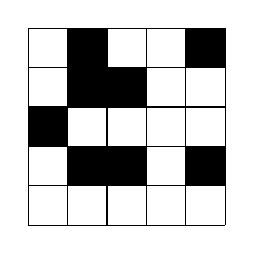
\begin{tikzpicture}[scale=0.5]
\fill[black] (1,1) rectangle (2,2);
\fill[black] (1,4) rectangle (2,5);
\fill[black] (4,1) rectangle (5,2);
\fill[black] (4,4) rectangle (5,5);
\fill[black] (1,3) rectangle (2,4);
\fill[black] (2,3) rectangle (3,4);
\fill[black] (2,1) rectangle (3,2);
\fill[black] (0,2) rectangle (1,3);
\draw (0,0) grid (5,5);
\end{tikzpicture}
\end{center}
包含两个这样的子网格：
\begin{center}
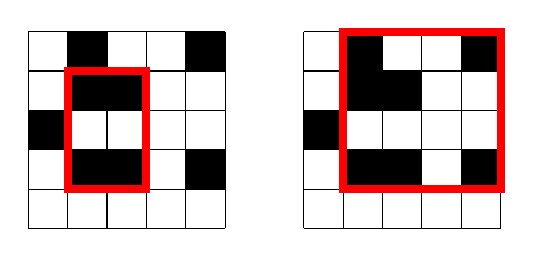
\begin{tikzpicture}[scale=0.5]
\fill[black] (1,1) rectangle (2,2);
\fill[black] (1,4) rectangle (2,5);
\fill[black] (4,1) rectangle (5,2);
\fill[black] (4,4) rectangle (5,5);
\fill[black] (1,3) rectangle (2,4);
\fill[black] (2,3) rectangle (3,4);
\fill[black] (2,1) rectangle (3,2);
\fill[black] (0,2) rectangle (1,3);
\draw (0,0) grid (5,5);

\fill[black] (7+1,1) rectangle (7+2,2);
\fill[black] (7+1,4) rectangle (7+2,5);
\fill[black] (7+4,1) rectangle (7+5,2);
\fill[black] (7+4,4) rectangle (7+5,5);
\fill[black] (7+1,3) rectangle (7+2,4);
\fill[black] (7+2,3) rectangle (7+3,4);
\fill[black] (7+2,1) rectangle (7+3,2);
\fill[black] (7+0,2) rectangle (7+1,3);
\draw (7+0,0) grid (7+5,5);

\draw[color=red,line width=1mm] (1,1) rectangle (3,4);
\draw[color=red,line width=1mm] (7+1,1) rectangle (7+5,5);
\end{tikzpicture}
\end{center}

有一个 $O(n^3)$ 时间的算法可以解决这个问题：
遍历所有 $O(n^2)$ 对行，
对于每一对 $(a,b)$，在 $O(n)$ 时间内计算两行中
同时为黑色的列数。
以下代码假设 $\texttt{color}[y][x]$
表示第 $y$ 行第 $x$ 列的颜色：
\begin{lstlisting}
int count = 0;
for (int i = 0; i < n; i++) {
    if (color[a][i] == 1 && color[b][i] == 1) count++;
}
\end{lstlisting}
那么，这些列构成了 $\texttt{count}(\texttt{count}-1)/2$ 个黑色角的子网格，
因为我们可以从它们中任意选择两个来组成一个子网格。

为了优化这个算法，我们将网格划分为列的块，
每个块由 $N$ 个连续的列组成。然后，
每一行存储为一系列 $N$ 位数，描述各格子的颜色。
现在我们可以使用位运算同时处理 $N$ 列。
在以下代码中，
$\texttt{color}[y][k]$ 表示
一个 $N$ 位的颜色块。
\begin{lstlisting}
int count = 0;
for (int i = 0; i <= n/N; i++) {
    count += __builtin_popcount(color[a][i]&color[b][i]);
}
\end{lstlisting}
得到的算法的工作时间为 $O(n^3/N)$。

我们生成了一个大小为 $2500 \times 2500$ 的随机网格，
并比较了原始实现和位优化实现。
原始代码花费了 $29.6$ 秒，
而位优化版本在 $N=32$（\texttt{int} 数）时仅花费了 $3.1$ 秒，
在 $N=64$（\texttt{long long} 数）时花费了 $1.7$ 秒。

\section{动态规划}

位运算提供了一种高效且便捷的方式
来实现状态包含元素子集的动态规划算法，
因为这样的状态可以存储为整数。
接下来我们讨论位运算与动态规划结合的示例。

\subsubsection{最优选择}

作为第一个例子，考虑以下问题：
给定 $k$ 种产品在 $n$ 天内的价格，
我们希望每种产品都恰好购买一次。
但每天最多只能购买一种产品。
最小总价格是多少？
例如，考虑以下场景（$k=3$ 且 $n=8$）：
\begin{center}
\begin{tikzpicture}[scale=.65]
    \draw (0, 0) grid (8,3);
    \node at (-2.5,2.5) {产品 0};
    \node at (-2.5,1.5) {产品 1};
    \node at (-2.5,0.5) {产品 2};

    \foreach \x in {0,...,7}
        {\node at (\x+0.5,3.5) {\x};}
    \foreach \x/\v in {0/6,1/9,2/5,3/2,4/8,5/9,6/1,7/6}
        {\node at (\x+0.5,2.5) {\v};}
    \foreach \x/\v in {0/8,1/2,2/6,3/2,4/7,5/5,6/7,7/2}
        {\node at (\x+0.5,1.5) {\v};}
    \foreach \x/\v in {0/5,1/3,2/9,3/7,4/3,5/5,6/1,7/4}
        {\node at (\x+0.5,0.5) {\v};}
\end{tikzpicture}
\end{center}
在这个场景中，最小总价格是 $5$：
\begin{center}
\begin{tikzpicture}[scale=.65]
    \fill [color=lightgray] (1, 1) rectangle (2, 2);
    \fill [color=lightgray] (3, 2) rectangle (4, 3);
    \fill [color=lightgray] (6, 0) rectangle (7, 1);
    \draw (0, 0) grid (8,3);
    \node at (-2.5,2.5) {产品 0};
    \node at (-2.5,1.5) {产品 1};
    \node at (-2.5,0.5) {产品 2};

    \foreach \x in {0,...,7}
        {\node at (\x+0.5,3.5) {\x};}
    \foreach \x/\v in {0/6,1/9,2/5,3/2,4/8,5/9,6/1,7/6}
        {\node at (\x+0.5,2.5) {\v};}
    \foreach \x/\v in {0/8,1/2,2/6,3/2,4/7,5/5,6/7,7/2}
        {\node at (\x+0.5,1.5) {\v};}
    \foreach \x/\v in {0/5,1/3,2/9,3/7,4/3,5/5,6/1,7/4}
        {\node at (\x+0.5,0.5) {\v};}
\end{tikzpicture}
\end{center}

设 $\texttt{price}[x][d]$ 表示产品 $x$
在第 $d$ 天的价格。
例如，在上述场景中 $\texttt{price}[2][3] = 7$。
然后，设 $\texttt{total}(S,d)$ 表示在第 $d$ 天之前
购买产品子集 $S$ 的最小总价格。
使用这个函数，问题的解是
$\texttt{total}(\{0 \ldots k-1\},n-1)$。

首先，$\texttt{total}(\emptyset,d) = 0$，
因为购买空集不需要任何花费，
而 $\texttt{total}(\{x\},0) = \texttt{price}[x][0]$，
因为在第一天购买一种产品只有一种方式。
然后，可以使用以下递推关系：
\begin{equation*}
\begin{split}
\texttt{total}(S,d) = \min( & \texttt{total}(S,d-1), \\
& \min_{x \in S} (\texttt{total}(S \setminus x,d-1)+\texttt{price}[x][d]))
\end{split}
\end{equation*}
这意味着我们在第 $d$ 天要么不购买任何产品，
要么购买属于 $S$ 的某种产品 $x$。
在后一种情况下，我们将 $x$ 从 $S$ 中移除，
并将 $x$ 的价格加到总价格中。

下一步是使用动态规划来计算函数的值。
为了存储函数值，我们声明一个数组
\begin{lstlisting}
int total[1<<K][N];
\end{lstlisting}
其中 $K$ 和 $N$ 是足够大的常数。
数组的第一维对应于子集的位表示。

首先，$d=0$ 的情况可以如下处理：
\begin{lstlisting}
for (int x = 0; x < k; x++) {
    total[1<<x][0] = price[x][0];
}
\end{lstlisting}
然后，递推关系转换为以下代码：
\begin{lstlisting}
for (int d = 1; d < n; d++) {
    for (int s = 0; s < (1<<k); s++) {
        total[s][d] = total[s][d-1];
        for (int x = 0; x < k; x++) {
            if (s&(1<<x)) {
                total[s][d] = min(total[s][d],
                                    total[s^(1<<x)][d-1]+price[x][d]);
            }
        }
    }
}
\end{lstlisting}
算法的时间复杂度为 $O(n 2^k k)$。

\subsubsection{从排列到子集}

使用动态规划，通常可以将对排列的遍历
转换为对子集的遍历\footnote{这个技术由 M. Held 和 R. M. Karp 于1962年引入 \cite{hel62}。}。
这样做的好处是排列数 $n!$
远大于子集数 $2^n$。
例如，如果 $n=20$，则
$n! \approx 2.4 \cdot 10^{18}$，而 $2^n \approx 10^6$。
因此，对于某些 $n$ 的值，
我们可以高效地遍历子集但不能遍历排列。

作为一个例子，考虑以下问题：
有一部最大承重为 $x$ 的电梯，
和 $n$ 个已知体重的人，
他们想从底层到达顶层。
如果人们以最优顺序进入电梯，
最少需要多少次搭乘电梯？

例如，假设 $x=10$，$n=5$，
体重如下：
\begin{center}
\begin{tabular}{ll}
人 & 体重 \\
\hline
0 & 2 \\
1 & 3 \\
2 & 3 \\
3 & 5 \\
4 & 6 \\
\end{tabular}
\end{center}
在这种情况下，最少需要2次。
一个最优顺序是 $\{0,2,3,1,4\}$，
将人分为两次：
先是 $\{0,2,3\}$（总重10），
然后是 $\{1,4\}$（总重9）。

这个问题可以在 $O(n! n)$ 时间内轻松解决，
方法是枚举 $n$ 个人的所有可能排列。
但我们可以使用动态规划来获得
更高效的 $O(2^n n)$ 时间算法。
思路是为每个人的子集计算两个值：
所需的最少次数和最后一次中人的最小体重。

设 $\texttt{weight}[p]$ 表示人 $p$ 的体重。
我们定义两个函数：
$\texttt{rides}(S)$ 是子集 $S$ 所需的
最少次数，
$\texttt{last}(S)$ 是最后一次的最小体重。
例如，在上述场景中
\[ \texttt{rides}(\{1,3,4\})=2 \hspace{10pt} \textrm{和}
\hspace{10pt} \texttt{last}(\{1,3,4\})=5,\]
因为最优的乘梯分配是 $\{1,4\}$ 和 $\{3\}$，
且第二次的体重是5。
当然，我们的最终目标是计算
$\texttt{rides}(\{0 \ldots n-1\})$ 的值。

我们可以递归地计算函数的值，
然后应用动态规划。
思路是遍历属于 $S$ 的所有人，
并最优地选择最后进入电梯的人 $p$。
每种选择都会产生一个
更小子集的子问题。
如果 $\texttt{last}(S \setminus p)+\texttt{weight}[p] \le x$，
我们可以将 $p$ 加入最后一次。
否则，我们需要开辟新的一次，
最初只包含 $p$。

为了实现动态规划，
我们声明一个数组
\begin{lstlisting}
pair<int,int> best[1<<N];
\end{lstlisting}
对于每个子集 $S$，
它包含一个对 $(\texttt{rides}(S),\texttt{last}(S))$。
我们将空组的值设置如下：
\begin{lstlisting}
best[0] = {1,0};
\end{lstlisting}
然后，我们可以如下填充数组：

\begin{lstlisting}
for (int s = 1; s < (1<<n); s++) {
    // 初始值：需要 n+1 次
    best[s] = {n+1,0};
    for (int p = 0; p < n; p++) {
        if (s&(1<<p)) {
            auto option = best[s^(1<<p)];
            if (option.second+weight[p] <= x) {
                // 将 p 加入现有的一次
                option.second += weight[p];
            } else {
                // 为 p 开辟新的一次
                option.first++;
                option.second = weight[p];
            }
            best[s] = min(best[s], option);
        }
    }
}
\end{lstlisting}
注意，上述循环保证了
对于任意两个子集 $S_1$ 和 $S_2$，
如果 $S_1 \subset S_2$，则先处理 $S_1$ 再处理 $S_2$。
因此，动态规划的值是以正确的顺序计算的。

\subsubsection{计数子集}

本章的最后一个问题如下：
设 $X=\{0 \ldots n-1\}$，每个子集 $S \subset X$
被赋予一个整数值 $\texttt{value}[S]$。
我们的任务是对每个 $S$ 计算
\[\texttt{sum}(S) = \sum_{A \subset S} \texttt{value}[A],\]
即 $S$ 的所有子集的值之和。

例如，假设 $n=3$，值如下：
\begin{multicols}{2}
\begin{itemize}
\item $\texttt{value}[\emptyset] = 3$
\item $\texttt{value}[\{0\}] = 1$
\item $\texttt{value}[\{1\}] = 4$
\item $\texttt{value}[\{0,1\}] = 5$
\item $\texttt{value}[\{2\}] = 5$
\item $\texttt{value}[\{0,2\}] = 1$
\item $\texttt{value}[\{1,2\}] = 3$
\item $\texttt{value}[\{0,1,2\}] = 3$
\end{itemize}
\end{multicols}
在这种情况下，例如，
\begin{equation*}
\begin{split}
\texttt{sum}(\{0,2\}) &= \texttt{value}[\emptyset]+\texttt{value}[\{0\}]+\texttt{value}[\{2\}]+\texttt{value}[\{0,2\}] \\ 
                      &= 3 + 1 + 5 + 1 = 10.
\end{split}
\end{equation*}

因为总共有 $2^n$ 个子集，
一种可能的解决方案是在 $O(2^{2n})$ 时间内
遍历所有子集对。
然而，使用动态规划，
我们可以在 $O(2^n n)$ 时间内解决问题。
思路是聚焦于这样的求和：
其中可以从 $S$ 中移除的元素是受限的。

设 $\texttt{partial}(S,k)$ 表示 $S$ 的子集的值之和，
限制条件是只能从 $S$ 中
移除元素 $0 \ldots k$。
例如，
\[\texttt{partial}(\{0,2\},1)=\texttt{value}[\{2\}]+\texttt{value}[\{0,2\}],\]
因为我们只能移除元素 $0 \ldots 1$。
我们可以使用 \texttt{partial} 的值
来计算 \texttt{sum} 的值，因为
\[\texttt{sum}(S) = \texttt{partial}(S,n-1).\]
函数的基准情况是
\[\texttt{partial}(S,-1)=\texttt{value}[S],\]
因为在这种情况下不能从 $S$ 中移除任何元素。
然后，在一般情况下，我们可以使用以下递推关系：
\begin{equation*}
    \texttt{partial}(S,k) = \begin{cases}
               \texttt{partial}(S,k-1) & k \notin S \\
               \texttt{partial}(S,k-1) + \texttt{partial}(S \setminus \{k\},k-1) & k \in S
           \end{cases}
\end{equation*}
这里我们聚焦于元素 $k$。
如果 $k \in S$，我们有两个选择：
要么将 $k$ 保留在 $S$ 中，
要么将其从 $S$ 中移除。

有一种特别巧妙的方法来实现求和计算。
我们可以声明一个数组
\begin{lstlisting}
int sum[1<<N];
\end{lstlisting}
它将包含每个子集的和。
数组初始化如下：
\begin{lstlisting}
for (int s = 0; s < (1<<n); s++) {
    sum[s] = value[s];
}
\end{lstlisting}
然后，我们可以如下填充数组：
\begin{lstlisting}
for (int k = 0; k < n; k++) {
    for (int s = 0; s < (1<<n); s++) {
        if (s&(1<<k)) sum[s] += sum[s^(1<<k)];
    }
}
\end{lstlisting}
这段代码将 $\texttt{partial}(S,k)$
（$k=0 \ldots n-1$）的值计算到数组 \texttt{sum} 中。
由于 $\texttt{partial}(S,k)$ 总是基于
$\texttt{partial}(S,k-1)$，我们可以复用数组
\texttt{sum}，从而得到一个非常高效的实现。